\documentclass{beamer}
\title{Extending Zero Trust architecture to Kubernetes sidecars}
\author{Aarni Halinen}
\institute{
  Department of Computer Science\\
  Aalto University
}
\date{\today}

\begin{document}

\frame{
  \titlepage

  Supervisor: Prof.\ Mario Di Francesco
  \\
  Advisor: M.Sc.\ (Tech.)\ José\ Luis\ Martin\ Navarro
  \\
  Advisor: M.Sc.\ (Tech.)\ Jacopo\ Bufalino
}

\frame{
  \frametitle{Contents}

  \begin{enumerate}
    \item Zero Trust Architecture
    \item Kubernetes: sidecars and networking model
    \item Research: threat modeling and mitigation
    \item Future considerations
  \end{enumerate}
}

\frame{
  \frametitle[ZTA]{Zero Trust Architecture (ZTA)}

  \emph{A security paradigm that focuses on the premise that trust must always be explicitly granted}
  \begin{itemize}
    \item Move security boundaries to the most granular level and use fine-grained access rules
    \item A multi-layer, defense-in-depth approach
    \item Network communication, even if internal and behind a firewall, should not be trusted
    \item Services communicate securely (Mutual authentication, with mTLS), rely on more robust identifiers than IP addresses, and restrict traffic on L5-L7
    \item Service meshes help implementing ZTA in Kubernetes clusters, often using sidecars (like Envoy proxy)
  \end{itemize}
}

\frame{
  \frametitle{Kubernetes sidecar containers}

  \begin{itemize}
    \item Pods are the basic scheduling abstraction
    \begin{itemize}
      \item Consist of one or more tightly-coupled containers
      \item Share Linux network namespace
      \item Common lifecycle
    \end{itemize}
    \item Sidecar pattern allows isolating of peripheral tasks (logging, observability, Envoy proxies) from application to own helper containers
    \item Sidecars are not technically different from other containers
  \end{itemize}
}

\frame{
  \frametitle{K8s networking model}

  \begin{itemize}
    \item Addresses 4 different types of networking communication
    \begin{itemize}
      \item Inside Pod's network namespace (localhost)
      \item Pod-to-Pod, even accross different Nodes
      \item Service-to-Pod
      \item Cluster external sources to Services
    \end{itemize}
    \item Pod-to-Pod connection is implemented by a CNI plugin that creates NIC and assigns IP addresses (IPAM)
    \item CNI plugins with operator daemons can also implement network rules (Network Policy or Custom Resource Definition)
    \item Calico and Cilium are examples of mature CNI plugins
    \item Meta-plugins such as Multus implement other features as part of the CNI chain
  \end{itemize}
}

\frame{
  \frametitle{Research: Sidecar threat modeling}

  \begin{figure}[h!]
    \centering
    \includegraphics[width=\linewidth]{../thesis/files/Matrix copy.png}
    \caption{Microsoft's Threat Matrix for Kubernetes (adopted from MITRE ATT\&CK) [1]}
  \end{figure}

  \begin{itemize}
    \item Threat matrix used as the main source
    \item Attacks are also experimented with custom container in a Minikube cluster
  \end{itemize}
}

\frame{
  \frametitle{Sidecar threat modeling}

  \begin{itemize}
    \item Pods are the most granular security boundary of Kubernetes
    \item Sidecars inherit execution and networking privileges from the Pod
    \item $\Rightarrow$ Principle of least privilege is not respected
    \item $\Rightarrow$ Custom solutions are needed for container-level Zero Trust
  \end{itemize}
}

\frame{
  \frametitle{Configuration related threats}

  \begin{itemize}
    \item Most of the threats found are easily mitigated with Pod Security Admission Controller
    \item Other threats can be mitigated with custom admission controllers (Validating and mutating webhooks)
    \begin{itemize}
      \item Containers in a Pod share and automatically mount Service Accounts
      \item $\Rightarrow$ Disable automatic SA mounting, manually mount when needed
      \item Resource limits are not enforced by PSA (denial of service)
      \item Custom ValidatingAdmissionWebhook can be used for enforcement
    \end{itemize}
  \end{itemize}
}

\frame{
  \frametitle{Networking threats}

  \begin{itemize}
    \item Two main issues found:
    \begin{itemize}
      \item The common network namespace allows unlimited access to other containers in the Pod
      \item Network policies apply to all containers in a Pod
    \end{itemize}
    \item No built-in solution for fine-grained network access
    \item Loopback device is managed by container runtime $\Rightarrow$ Network Policies are not applicable
    \item Two different approaches invistigated
    \item Neither should interfere with Admission Controller
  \end{itemize}
}

\frame{
  \frametitle{Approach 1: Injecting networking rules to Pod}

  \begin{figure}[h!]
    \centering
    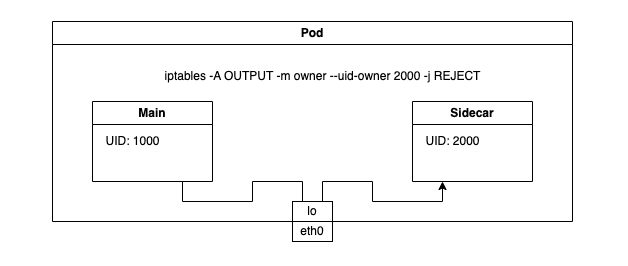
\includegraphics[width=\linewidth]{../thesis/files/iptables.png}
  \end{figure}

  \begin{itemize}
    \item Inject IPTables rules to Pod net namespace after deployment
    \item Containers are distinguished from one another by using unique user IDs and IPTables owner-module
  \end{itemize}
}

\frame{
  \frametitle{Approach 2: Split the Pod and rebuild sidecar-like connectivity}

  \begin{figure}[h!]
    \centering
    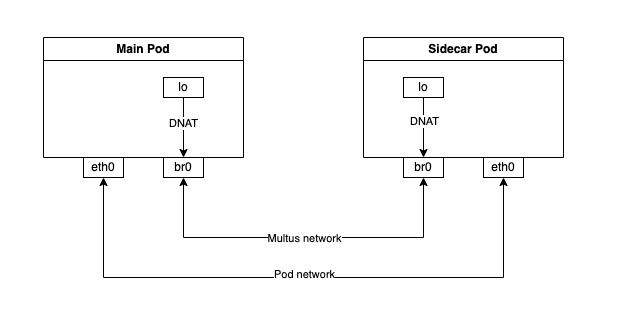
\includegraphics[width=\linewidth]{../thesis/files/multus.png}
  \end{figure}

  \begin{itemize}
    \item All containers are inherently in own net NS
    \item Multus used for static IPs, Network Policies and isolation from Pod network
    \item Route loopback to Multus network
    % \texttt{net.ipv4.conf.all.route\_localnet=1})
  \end{itemize}
}

\frame{
  \frametitle{Findings}

  \begin{itemize}
    \item Moving security boundaries to container-level is possible, but laborous to implement
    \begin{itemize}
      \item Keeping access rules up-to-date requires a custom K8s operator
      \item Multus is not yet a mature project
      \item Multus approach breaks co-scheduling and shared lifecycle
      \item mTLS and Multus are not compatible
    \end{itemize}
    \item \emph{Avoiding sidecars is the best mitigation}
    \item $\Rightarrow$ Use DaemonSets to run sidecars per-Node
  \end{itemize}
}

\frame{
  \frametitle{Future development}

  \begin{itemize}
    \item K8s v1.28 introduces SidecarContainers
    \begin{itemize}
      \item Introduced for fixing existing lifecycle issues of initContainers
      \item Proposal explicitly states a non-goal of enforcing different security regulations for sidecars
    \end{itemize}
    \item Service meshes have introduced sidecarless architectures
    \item Cilium service mesh (eBPF) and Istio ambient mesh
  \end{itemize}
}

\frame{
\frametitle{Re-cap}

\begin{figure}[h!]
  \centering
  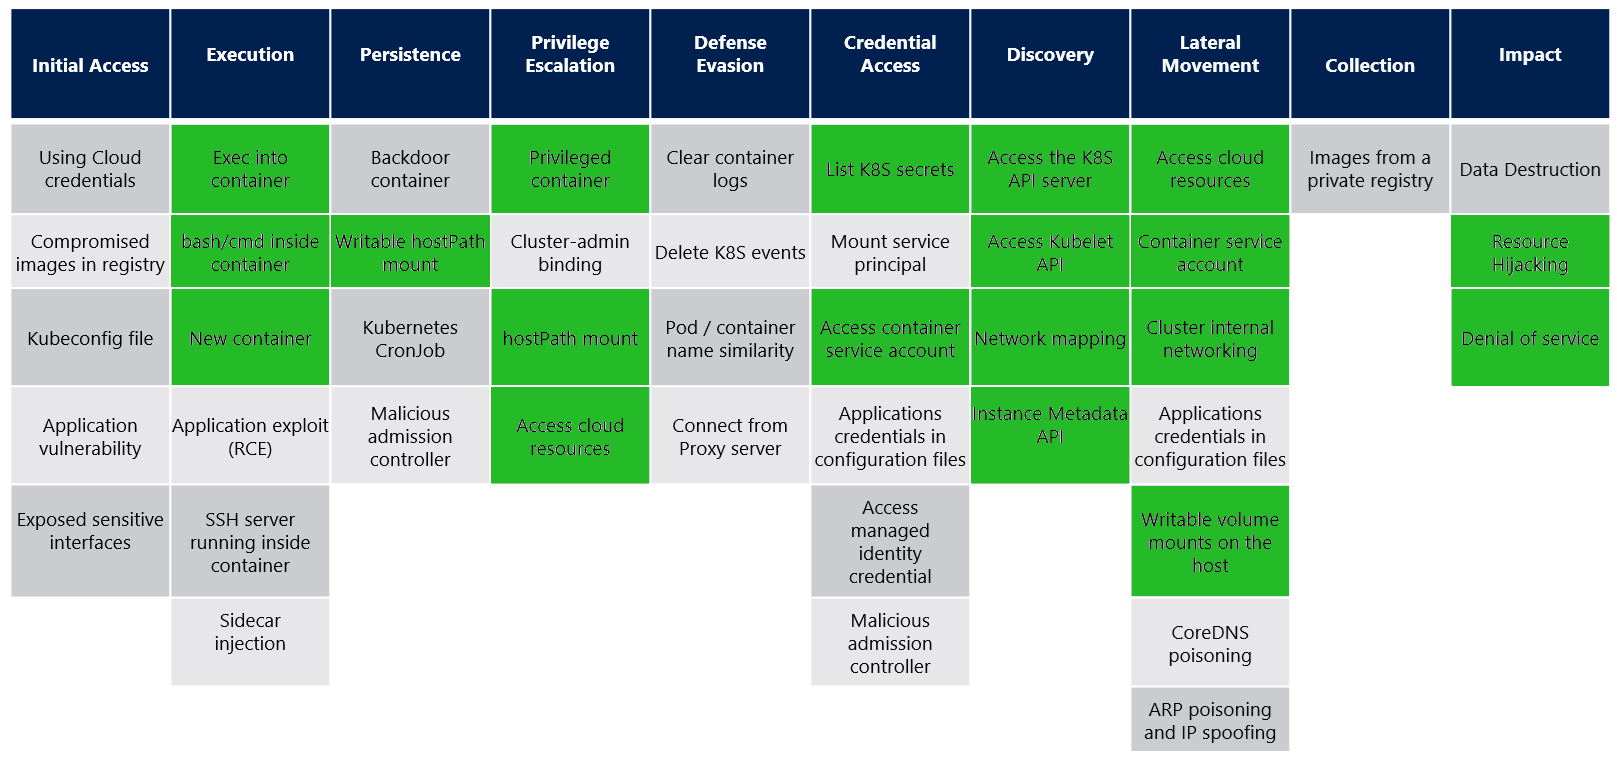
\includegraphics[width=\linewidth]{../thesis/files/Matrix.png}
  \caption{Threat matrix. Attack techniques addressed are highlighted in green.}
\end{figure}
}

\frame{
  \frametitle{Re-cap}

  \begin{itemize}
    \item The thesis investigated and found ways to mitigate sidecar related threats in K8s
    \item Most vulnerable configuration can be prevented with PSA
    \item Admission controller allows extending protections even further
    \item No existing way to implement ZTA in sidecar networking, but it is possible
    \item Implementing the network solutions are cumbersome and require extensive work
    \item Avoiding sidecars altogether is the easiest mitigation
  \end{itemize}
}

\frame{
  \frametitle{References}

  Experimental solutions can be found in Github repository: https://github.com/Arskah/k8s-sidecar-security

  \begin{itemize}
    \item [1] Secure containerized environments with updated threat matrix for Kubernetes, By Yossi Weizman, Senior Security Researcher, Microsoft Defender for Cloud.
    [https://www.microsoft.com/en-us/security/blog/2021/03/23/secure-containerized-environments-with-updated-threat-matrix-for-kubernetes/]
  \end{itemize}
}

\end{document}
